\documentclass{article}

%-------------------------------------------------

\usepackage{graphicx}

\usepackage{amsmath}
\usepackage{amssymb}
\usepackage{amsfonts}

\usepackage{color}

\usepackage{verbatim}

\usepackage{tikz}
\usetikzlibrary{arrows,automata}

%-------------------------------------------------

\newcommand{\GraceDB}{\texttt{GraceDB}~}
\newcommand{\alert}{\texttt{lvalert}~}

\newcommand{\lvalertListenMP}{\texttt{lvalert\_listenMP}~}
\newcommand{\lvalertCommandMP}{\texttt{lvalert\_commandMP}~}

\newcommand{\interactiveQueue}{\texttt{interactiveQueue}~}
\newcommand{\parseAlert}{\texttt{parseAlert}~}

\newcommand{\SortedQueue}{\texttt{SortedQueue}~}
\newcommand{\QueueItem}{\texttt{QueueItem}~}
\newcommand{\Task}{\texttt{Task}~}

\newcommand{\lvalertMPini}{\texttt{lvalert\_listenMP.ini}~}
\newcommand{\childConfigini}{\texttt{childConfig.ini}~}

%-------------------------------------------------
\begin{document}
%-------------------------------------------------

\title{
lvalertMP User's Guide
}

\author{
Reed Essick \\
reed.essick@ligo.org
}

\maketitle

%------------------------

\section{introduction}

\begin{itemize}
    \item{describe the problem this is meant to address}
    \item{describe how we solve the problem (change the format of the delegation but not the general idea)}
\end{itemize}

%------------------------

\section{classes, methods, configs and executables}

%-----------

\subsection{classes}

\subsubsection{\SortedQueue}

\subsubsection{\QueueItem}

\subsubsection{\Task}

%-----------

\subsection{methods}

\subsubsection{\interactiveQueue}

\subsubsection{\parseAlert}

%-----------

\subsection{configs}

\subsubsection{\lvalertMPini}

\subsubsection{\childConfigini}

%-----------

\subsection{executables}

\subsubsection{\lvalertListenMP}

\subsubsection{\lvalertCommandMP}

%------------------------

\section{workflow}

\begin{figure}
    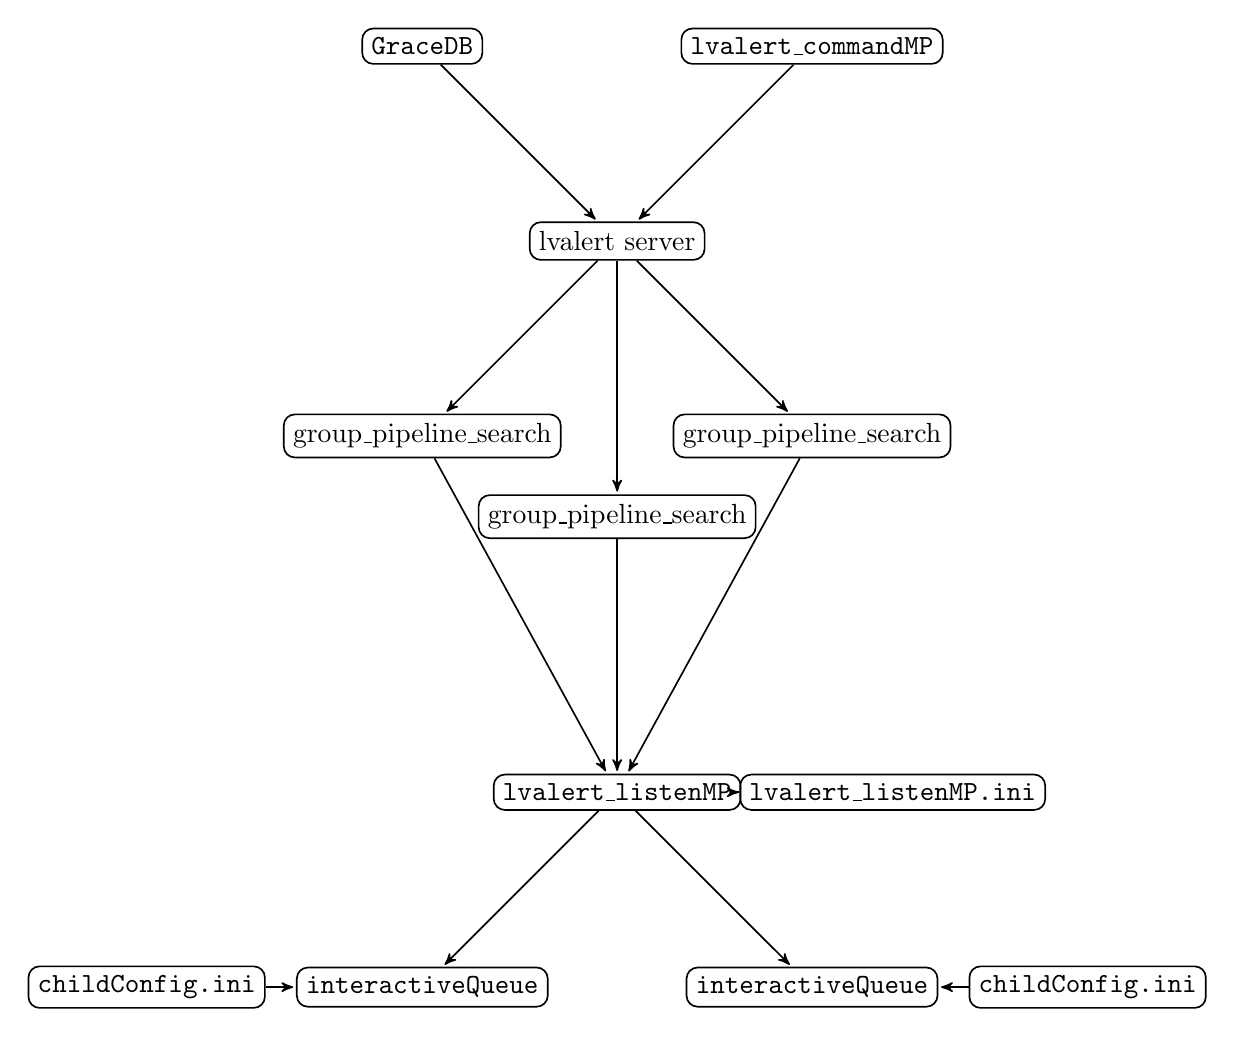
\begin{tikzpicture}[->,>=stealth', shorten >= 1pt, auto, node distance=3.50cm, semithick]
        \tikzset{
           server/.style={
                        rectangle,
                        rounded corners,
                        draw=black,
                        fill=none,
                        text=black
                       },
           lvalertNode/.style={
                        rectangle,
                        rounded corners,
                        draw=black,
                        fill=none,
                        text=black
                       },
           mpPipe/.style={
                        rectangle,
                        rounded corners,
                        draw=black,
                        fill=none,
                        text=black
                       },
           lvalertMP/.style={
                        rectangle,
                        rounded corners,
                        draw=black,
                        fill=none,
                        text=black
                       },
           config/.style={
                        rectangle,
                        rounded corners,
                        draw=black,
                        fill=none,
                        text=black
                       },
           childProc/.style={
                        rectangle,
                        rounded corners,
                        draw=black,
                        fill=none,
                        text=black
                       },
                 };
    %--------------------
        \node[server]      (lvalertServer)                                {lvalert server};

        \node[server]      (GraceDB)       [above left of=lvalertServer]  {\GraceDB};
        \node[lvalertMP]   (lvalertCmd)    [above right of=lvalertServer] {\lvalertCommandMP};

        \node[lvalertNode] (nodeA)         [below left of=lvalertServer]  {group\_pipeline\_search};
        \node[lvalertNode] (nodeB)         [below of=lvalertServer]       {group\_pipeline\_search};
        \node[lvalertNode] (nodeC)         [below right of=lvalertServer] {group\_pipeline\_search};

        \node[lvalertMP]   (lvalertMP)     [below of=nodeB]               {\lvalertListenMP};
        \node[config]      (lvalertConfig) [right of=lvalertMP]           {\lvalertMPini};

        \node[childProc]   (childProc1)    [below left of=lvalertMP]      {\interactiveQueue};
        \node[config]      (childConfig1)  [left of=childProc1]           {\childConfigini};
        \node[childProc]   (childProc2)    [below right of=lvalertMP]     {\interactiveQueue};
        \node[config]      (childConfig2)  [right of=childProc2]          {\childConfigini};
    %--------------------
        \path (GraceDB)       edge (lvalertServer)
              (lvalertCmd)    edge (lvalertServer)

              (lvalertServer) edge (nodeA)
              (lvalertServer) edge (nodeB)
              (lvalertServer) edge (nodeC)

              (nodeA)         edge (lvalertMP)
              (nodeB)         edge (lvalertMP)
              (nodeC)         edge (lvalertMP)

              (lvalertConfig) edge (lvalertMP)

              (lvalertMP)     edge (childProc1)
              (lvalertMP)     edge (childProc2)

              (childConfig1)  edge (childProc1)
              (childConfig2)  edge (childProc2);
    \end{tikzpicture}
    \caption{The flow of \alert messages between processes.}
    \label{fig: alert flow}
\end{figure}

%------------------------

\begin{figure}

\begin{verbatim}
queue = \SortedQueue()
queueByGID = {} <--- explain why we have both queue and queueByGID

while True:
    is there a new alert in the mpPipe?
        parseAlert( queue, queueByGID, alert, timeReceived )

    clean up / manage queue

    if queue[0].has_expired:
        item = queue.pop( 0 )
        item.execute() <--- show how QueueItems are structures and how execute() is delegated to Tasks
        if not item.complete:
            queue.insert( item )

    wait for a small amount of time before checking again
\end{verbatim}

    \caption{work flow within \interactiveQueue}
    \label{fig: interactiveQueue}
\end{figure}

\begin{figure}

    \caption{figure showing what happens within \parseAlert}
    \label{fig: parseAlert}
\end{figure}


%-------------------------------------------------
\end{document}
%-------------------------------------------------
